Dois arranjos serão estudados para o inversor monofásico: em semi-ponte e em ponte completa. Ambos podem ser observados na figura \ref{c1im}.

\begin{figure}[h]
\center
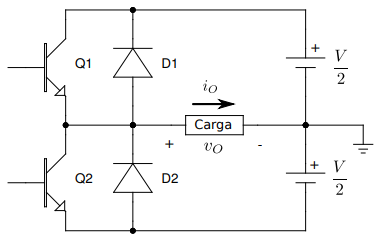
\includegraphics[scale=0.55]{imagens/circuito1_inversor_mono.png}
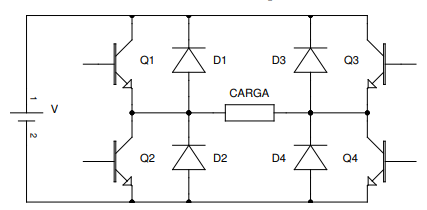
\includegraphics[scale=0.55]{imagens/circuito2_inversor_mono.png}
\caption{Circuitos de um inversor monofásico em semi-ponte. À esquerda, em semi-ponte;  direita em ponte completa.}\label{c1im} 
\caption*{Fonte: Apostila de eletrônica de potência (2015)}
\end{figure}

No caso da implementação em semi-ponte, através do chaveamento dos transistores Q1 e Q2 pode-se controlar a tensão observada pela carga. A figura \ref{g1im} ilustra esse comportamento. Não é difícil ver que se o controle de Q2 é replicado em Q3 e o de Q1 em Q4, temos o mesmo resultado, para a carga, no caso da implementação em ponte completa mas com amplitude dobrada. Nota-se que a tensão percebida pela carga é uma onda quadrada, mas simétrica e com frequência constante, desde que a frequência de chaveamento o seja.

\begin{figure}[h]
\center
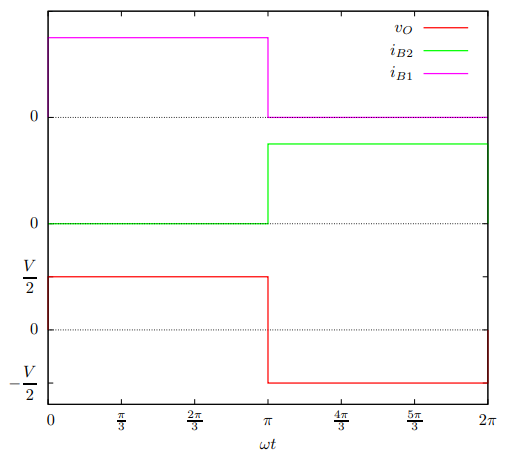
\includegraphics[scale=0.55]{imagens/grafico1_inversor_mono.png}
\caption{Tensão sobre a carga de um inversor monofásico em semi-ponte e correntes de acionamento dos transístores Q1 e Q2.}\label{g1im} 
\caption*{Fonte: Apostila de eletrônica de potência (2015)}
\end{figure}

Podemos, então, modelar a tensão de saída do inversor através da expansão em série de Fourier da onda quadrada gerada, i.e., \[
    v_{o} = \sum_{k=1}^{\infty}\frac{4A}{\left( 2k +1 \right) \pi}\sin{\left( 2k+1 \right) \omega{t}} 
,\] onde $A$ é a amplitude da tensão de saída (portanto $A = \frac{V}{2}$ para o inversor em semi-ponte e $A = V$ para o inversor em ponte completa), $\omega = 2\pi f$ é a frequência da tensão de saída.

Caso a carga seja puramente resistiva é evidente que a corrente possuirá o mesmo comportamento da tensão. No caso de uma carga com componente indutivo, a corrente na carga torna-se \[
    i_{o} = \sum_{k=1}^{\infty}\frac{4A}{\left( 2k+1 \right) \pi{|Z_{k}|}}\sin(\left( 2k+1 \right)\omega{t} - \phi_{k})
,\] onde $\tau = \frac{L}{R}$, $|Z_k| = \sqrt{R^{2} + (\left( 2k+1 \right) \omega{L})^2}$ e \[
\phi_{k} = \tan^{-1} \frac{\left( 2k+1 \right) \omega{L}}{R}
.\] 

Também pode-se escrever a corrente em função da amplitude $A$, de forma \[
i_o = \begin{cases}
    \frac{A}{R}(1-e^{-t/\tau}) &, t \in [0,\frac{T}{2}) \\
    \frac{-A}{R}(1-e^{-(t-\frac{T}{2})/\tau}) + I_{max}e^{-(t-\frac{T}{2})/\tau} &, t \in [\frac{T}{2},T)
\end{cases}
,\] onde: \[
    I_{MAX} = \frac{A}{R} \left(  \frac{1-e^{-\frac{T}{2\tau}}}{1+e^{-\frac{T}{2\tau}}}\right) 
.\]

Caso seja uma carga com componente capacitivo, a corrente pode ser descrita por \[
i_o = \begin{cases}
    I_{MAX}e^{-t/\tau} &, t \in \left[0,\frac{T}{2}\right) \\
    I_{MAX}e^{-(t-\frac{T}{2})/\tau} &, t \in \left[\frac{T}{2}, T\right)
\end{cases}
\] e a tensão \[
i_o = \begin{cases}
    A(1-e^{-t/\tau}) - V_{CO}e^{-t/\tau} &, t \in \left[0,\frac{T}{2}\right) \\
    A(1-e^{-(t-\frac{T}{2})/\tau}) + V_{C0}e^{-(t-\frac{T}{2})/\tau} &, t \in \left[\frac{T}{2}, T\right)
\end{cases}
,\] onde \[
    V_{C0} = A\frac{1-e^{-\frac{T}{2\tau}}}{1+e^{-\frac{T}{2\tau}}}
\] e \[
    I_{MAX} = \frac{A + V_{co}}{R}
.\]

A figura \ref{g3im} ilustra o comportamento da tensão e da corrente para ambas as cargas não lineares.

\begin{figure}[h]
\center
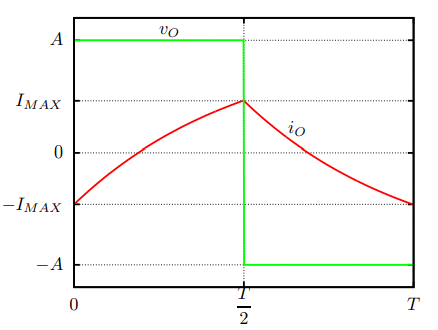
\includegraphics[scale=0.55]{imagens/grafico3_inversor_mono.png}
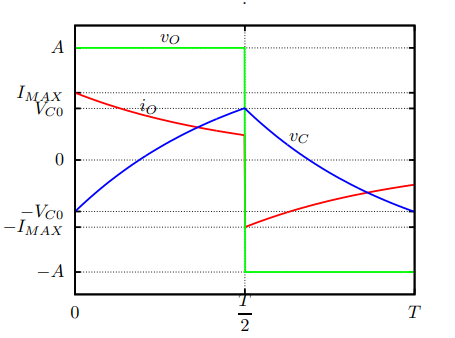
\includegraphics[scale=0.55]{imagens/grafico4_inversor_mono.png}
\caption{Corrente e tensão na carga de um inversor monofásico. À esquerda, carga RL; à direita, carga RC.}\label{g3im} 
\caption*{Fonte: Apostila de eletrônica de potência (2015)}
\end{figure}

